\documentclass[UTF8]{ctexart}
\usepackage[a4paper, top=25.4mm, bottom=25.4mm, left=31.8mm, right=31.8mm]{geometry}
\usepackage{graphicx}
\usepackage{amsmath}
\usepackage{multirow}
\usepackage{listings}
\usepackage{subcaption}
\usepackage{tabu}
\usepackage[T1]{fontenc}
\usepackage{booktabs}
\usepackage{minted}
\usemintedstyle{manni}
\usepackage[table]{xcolor}

\setlength{\parskip}{1em}
\definecolor{lightergray}{gray}{0.95}
\setlength{\tabcolsep}{12pt}
\renewcommand{\arraystretch}{1}
\lstset{
basicstyle=\ttfamily,
columns=flexible,
breaklines=true
}

\begin{document}
\begin{titlepage}
  \begin{center}
    \vspace*{1cm}

    \Large
    编译原理

    \vspace{0.5cm}
    \Huge
    \textbf{语法分析实验实验报告}

    \vfill

    \normalsize\kaishu
    班级:07111603 \\
    学号:1120161730 \\
    姓名:武上博 \\
    \today
    \vspace{1cm}
  \end{center}
\end{titlepage}

\tableofcontents
\newpage

\section{实验目的}
\begin{enumerate}
  \item 熟悉 C 语言的语法规则,了解编译器语法分析器的主要功能
  \item 熟练掌握典型语法分析器构造的相关技术和方法,设计并实现具有一定分析能力的 C 语言语法分析器
  \item 掌握编译器从前端到后端各个模块的工作原理,语法分析模块与其他模块之间的交互过程
\end{enumerate}

\section{实验内容}
\begin{enumerate}
  \item 该实验选择 C 语言的一个子集,基于 BIT-MiniCC 构建 C 语法子集的语法分析器,该语法分析器能够读入 XML 文件形式的属性字符流,进行语法分析并进行错误处理,如果输入正确时输出 XML 形式的语法树,输入不正确时报告语法错误。
  \item 将分析树转换为抽象语法树,便于后续分析工作和代码生成工作的完成。
\end{enumerate}

\section{实验的具体过程步骤}
\subsection{项目整体架构设计}
本次语法分析实验是在上一个词法分析实验的基础之上进行的,我们的大致要求是将词法分析得到的 Token 文件读入,作为语法分析的输入串,在通过语法分析器之后得到相应的语法树。经过考虑,我决定使用自顶向下的 LL(1) 语法分析方法。

LL(1) 语法分析器的具体架构是这样的:

\begin{itemize}
  \item 文法输入模块
  \item LL(1) 主控程序
  \begin{itemize}
    \item First 集合求解模块
    \item Follow 集合求解模块
    \item LL(1) 分析表构造模块
  \end{itemize}
  \item 输入串分析模块
\end{itemize}

为了和 BIT-MiniCC 框架进行结合,我们需要读入词法分析 Token 的 XML 文件作为我们的输入。同时我们需要输出符合规范的抽象语法树对应的 XML 文件作为下一步的输入。

我本次项目选择使用 Python 进行实现。我设计了:

\begin{itemize}
  \item \texttt{main.py}:LL(1) 分析器的主控程序,调用下面两个模块
  \item \texttt{parserUtils.py}:LL(1) 分析器的工具类,包含了对文法的读入、分析、First 和 Follow 集合的求取以及 LL(1) 分析表的求取等工具
  \item \texttt{parserGeneral.py}:LL(1) 分析器的主要模块,通过读入 Token 文件以及 LL(1) 分析表,得到语法分析树,并输出为合法的 XML 文件
\end{itemize}

这三个主要模块,构成了全部的 LL(1) 分析器。程序大致的流程如下图 \ref{fig:figure1}:

\begin{figure}[h]
  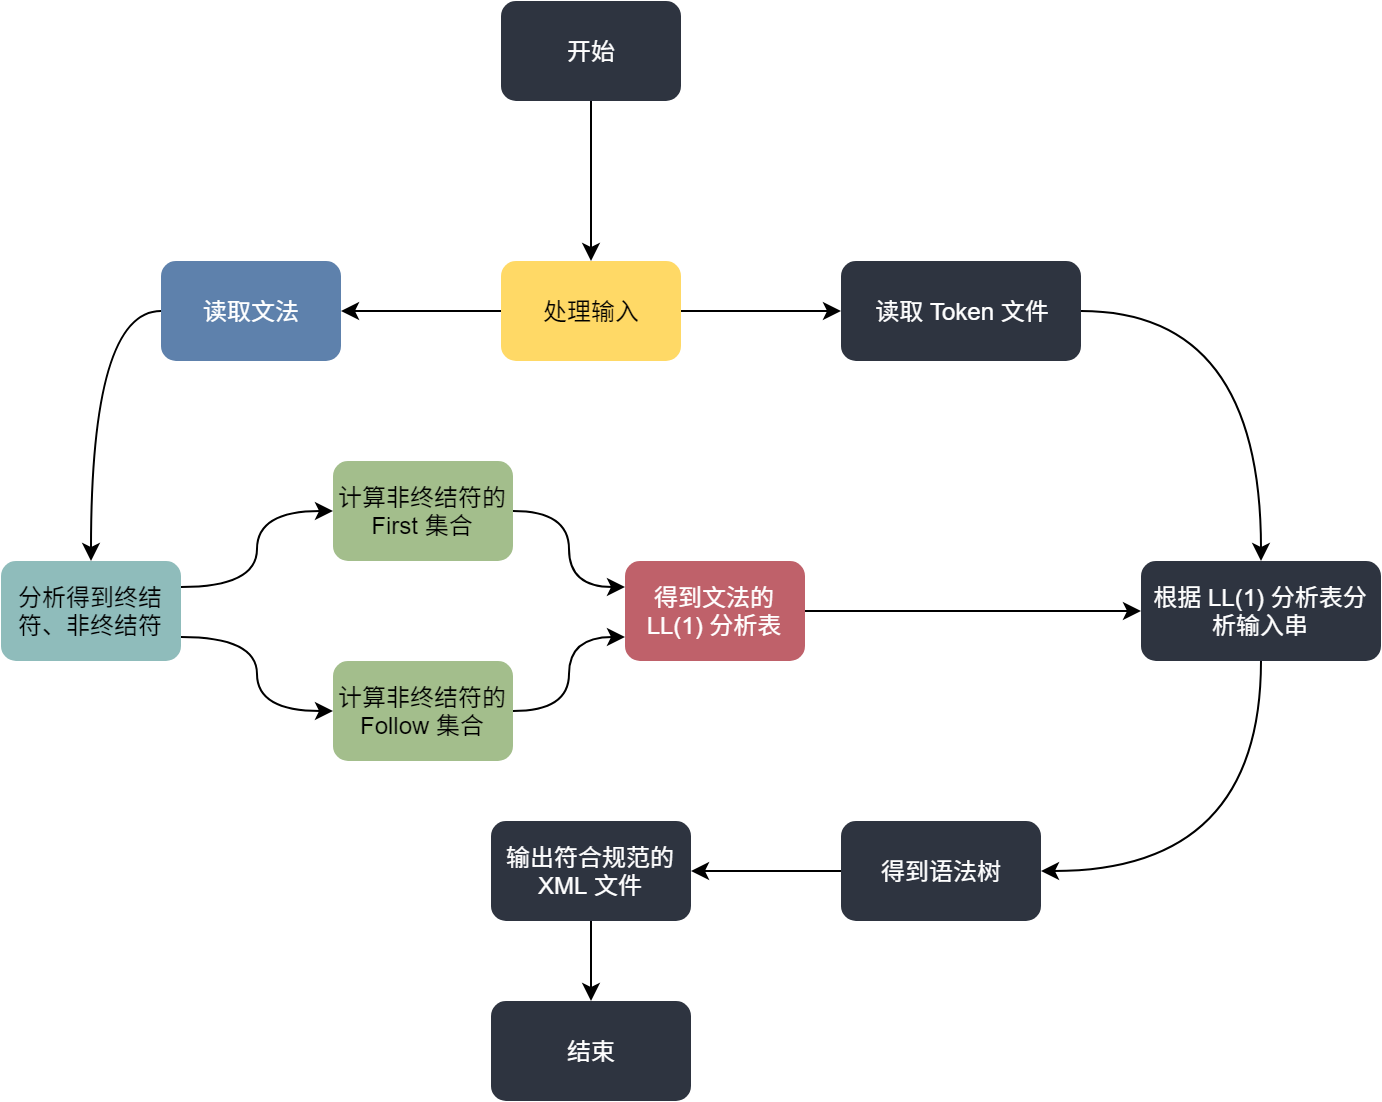
\includegraphics[width=\linewidth]{images/ll1.png}
  \caption{LL(1) 分析器的大致工作流程}
  \label{fig:figure1}
\end{figure}

\subsection{各个模块的具体实现}
接下来,我对每个模块的具体实现一一进行介绍。

\subsubsection{定义文法}
本次实验中,我在实验要求的文法基础之上,进行了一些扩展,增加了 C 语言中“声明语句”、“循环语句”、“判断语句”以及“跳转语句”的定义。同时,我也适当修改了原有的文法,包括对变量的声明、外部函数等等内容。本次实验中我所采用的全部文法如下所示:

\begin{lstlisting}
TRANSLATION_UNIT -> FUNCTION_DEFINITION
FUNCTION_DEFINITION -> TYPE_SPECIFIER identifier ( PARAM_LIST ) CODE_BLOCK
PARAM_LIST -> ARGUMENT | ARGUMENT , PARAM_LIST | empty
ARGUMENT -> TYPE_SPECIFIER identifier
TYPE_SPECIFIER -> int | float | short | long | void | double | char
CODE_BLOCK -> { STATEMENT_LIST }
STATEMENT_LIST -> STATEMENT STATEMENT_LIST | empty
STATEMENT -> DECLARATION_STATEMENT | ASSIGN_STATEMENT | RETURN_STATEMENT | LOOP_STATEMENT | SELECT_STATEMENT
DECLARATION_STATEMENT -> TYPE_SPECIFIER identifier ; | TYPE_SPECIFIER ASSIGN_STATEMENT
ASSIGN_STATEMENT -> identifier ASSIGN_OPERATOR EXPRESSION ;
ASSIGN_OPERATOR -> = | += | -= | *= | /= | ^= | %= | &=
RETURN_STATEMENT -> return EXPRESSION ;
JUMP_STATEMENT -> continue ; | break ; | goto identifier ;
LOOP_STATEMENT -> for ( EXPRESSION ; EXPRESSION ; EXPRESSION ) CODE_BLOCK | while ( EXPRESSION ) CODE_BLOCK | do CODE_BLOCK while ( EXPRESSION ) ;
SELECT_STATEMENT -> if ( EXPRESSION ) CODE_BLOCK | if ( EXPRESSION ) CODE_BLOCK else CODE_BLOCK | switch ( EXPRESSION ) CODE_BLOCK
EXPRESSION -> TERM EXPRESSION2 | empty
EXPRESSION2 -> + TERM EXPRESSION2 | - TERM EXPRESSION2 | empty
TERM -> FACTOR TERM2
TERM2 -> * FACTOR TERM2 | / FACTOR TERM2 | empty
FACTOR -> identifier | CONSTANT | ( EXPRESSION )
CONSTANT -> integer_constant | floating_constant | char | string
\end{lstlisting}

\subsubsection{输入文法,并以字典的形式存储}
为了方便存储文法,以 \texttt{FACTOR -> identifier | CONSTANT | (EXPRESSION)} 为例子,我按照如下的形式存储文法:

\begin{verbatim}
{
  'FACTOR': [['identifier'], ['CONSTANT'], ['(', 'EXPRESSION', ')']}
}
\end{verbatim}

可以看到,我将文法产生式左侧非终结符作为字典的 key,将相应的 value 定为文法后缀的生成式列表。我以 “\texttt{|}” 区分不同的生成式,这样就能够很好的对文法进行分析处理了。

相应的,在 Python 中,我使用了下面的方式对文法 \texttt{grammar} 进行初始化:

\begin{minted}[linenos,frame=lines,framesep=2mm]{python}
grammar = collections.defaultdict(list)
\end{minted}

之后,按行读入文法,并处理,最后得到“字典嵌套列表”的一个数据结构。

\begin{minted}[linenos,frame=lines,framesep=2mm]{python}
with open(filePath, 'r') as f:
    # 按行读取,加入文法字典
    for line in f:
      preGrammar, postGrammar = line.rstrip('\n').split('->')
      preGrammar = preGrammar.rstrip(' ')
      postGrammar = postGrammar.lstrip(' ').split('|')

      for eachPostGrammar in postGrammar:
        eachPostGrammar = eachPostGrammar.strip(' ').split(' ')
        grammar[preGrammar].append(eachPostGrammar)
\end{minted}

\subsubsection{处理终结符与非终结符}
对输入的文法进行遍历获取终结符与非终结符列表相对简单,只需要将文法生成式的前部加入非终结符集合,再遍历文法的后缀,如果遇到了不在非终结符集合中的符号,直接加入终结符集合即可。

\begin{minted}[linenos,frame=lines,framesep=2mm]{python}
def differentiateSymbols(grammar):
  # ...
  return terminalSymbols, nonTerminalSymbols
\end{minted}

通过上面两个步骤,我们已经成功的得到了文法的具体内容、文法的终结符与非终结符集合。这样,我们就可以利用这三个集合,通过接下来的算法构造 LL(1) 分析表。

\subsubsection{获取文法的 First 与 Follow 集合}
\paragraph{First 集合}
首先,我们对文法的每一项非终结符求取其 First 集合。First 集合是非终结符(或终结符、空符号串等等)的开始符号集合。对于文法 G 来说,G 中的 $\forall \alpha \in V^*$ 终结首符号集合 $FIRST(\alpha)$ 为:

\begin{equation}
  FIRST(\alpha) = \{a | \alpha^* \Rightarrow a, a \in V_T\}
\end{equation}

若 $a^* \Rightarrow \epsilon$,则 $\epsilon \in FIRST(\alpha)$。

在求取 First 集合时,我们是通过下面大致的代码描述进行求取的。

\begin{minted}[linenos,frame=lines,framesep=2mm]{python}
def getFIRST(firstSet, grammar, terminalSymbols, nonTerminalSymbols):
  for eachGrammar in grammar:
    for eachPostGrammar in grammar[eachGrammar]:
      # 1. 遇到了终结符、产生式右侧子式首符号是终结符,直接加入
      if ...
      # 2. 产生式右侧子式首符号,递归求取(比如:A -> B C c)
      else ...
  return firstSet
\end{minted}

为了保证 First 集合的完整性,我们需要递归多次求取文法的 First 集合。在主控程序循环求取 First 集合,直到两次求得的 First 集合相同即可停止。

\begin{minted}[linenos,frame=lines,framesep=2mm]{python}
grammarFirstSet = collections.defaultdict(list)
grammarFirstSet = parserUtils.getFIRST(
    grammarFirstSet, grammar, terminalSymbols, nonTerminalSymbols)
while True:
  originalFirstSet = copy.deepcopy(grammarFirstSet)
  grammarFirstSet = parserUtils.getFIRST(
      grammarFirstSet, grammar, terminalSymbols, nonTerminalSymbols)
  if grammarFirstSet == originalFirstSet:
    break
\end{minted}

\paragraph{Follow 集合}
在上一步骤 First 集合的基础之上,我们求取 Follow 集合。Follow 集合是对于文法 G 的所有句型中能够紧跟在非终结符号后面的一切终结符号(或者“\#”)。对上下文无关文法 G 来说,S 是文法的开始符号,对于文法 G 的任何非终结符号 A:

\begin{equation}
  FOLLOW(A) = \{ a | S^* \Rightarrow \dots Aa \dots, a \in V_T^* \}
\end{equation}

若 $S^* \Rightarrow \dots A$,则 $\# \in FOLLOW(A)$。

我们在构造 Follow 集合时,采用下面描述的算法:

\noindent\fbox{%
  \parbox{\linewidth}{%
对文法 G 中每个 $A \in V_N$:

\begin{enumerate}
  \item 对 G 的开始符号 S,令 $\# \in FOLLOW(S)$
  \item 如果文法 G 中出现了形如 $B \rightarrow \alpha A\beta$ 的产生式,且 $\beta \neq \epsilon$,则将 $FIRST(\beta)$ 中除了 $\epsilon$ 的符号全部加入 FOLLOW(A) 中
  \item 如果文法 G 中出现了形如 $B \rightarrow \alpha A$,或 $B \rightarrow \alpha A \beta$ 且 $\epsilon \in FIRST(\beta)$ 的产生式,则将 FOLLOW(B) 中全部内容加入 FOLLOW(A) 中
\end{enumerate}
  }%
}

在具体的代码实现中:

\begin{minted}[linenos,frame=lines,framesep=2mm]{python}
def getFOLLOW(
  firstSet, followSet, grammar, terminalSymbols, nonTerminalSymbols):
  for eachGrammarStartSymbol in grammar.keys():
    for eachGrammar in grammar:
      for eachPostGrammar in grammar[eachGrammar]:
        if eachGrammarStartSymbol in eachPostGrammar:
          # 1. 产生式形如:S->aX,将集合 Follow(S) 中的所有元素加入 Follow(X) 中
          if ...
          # 2. 产生式形如:S->aXb
          else ...
            # 2.1 b 为终结符:将 b 加入 Follow(X) 中
            if ...
            # 2.2 b 为非终结符
            else ...
  return followSet
\end{minted}

对于 Follow 集合,我们同样也需要通过递归求取的方式保证我们求得的 Follow 集合完整。在主控程序中,我们循环求取 Follow 集合,直到两次求得的 Follow 集合相同即可停止。

\begin{minted}[linenos,frame=lines,framesep=2mm]{python}
grammarTop = list(grammar.keys())[0]
grammarFollowSet = collections.defaultdict(list, {grammarTop: ['#']})
grammarFollowSet = parserUtils.getFOLLOW(
    grammarFirstSet, grammarFollowSet, grammar,
    terminalSymbols, nonTerminalSymbols)
while True:
  originalFollowSet = copy.deepcopy(grammarFollowSet)
  grammarFollowSet = parserUtils.getFOLLOW(
      grammarFirstSet, grammarFollowSet, grammar,
      terminalSymbols, nonTerminalSymbols)
  if grammarFollowSet == originalFollowSet:
    break
\end{minted}

\subsubsection{得到相应的 LL(1) 分析表}
从上面两步骤我们得到了文法的 First 和 Follow 集合。这一步我们可以开始对 LL(1) 分析表进行构造。分析表以 $M[A,a]$ 形式的矩阵来表示,A 是非终结符号,a 是文法的终结符号(或“\#”)。每一个矩阵的元素都存有一条关于非终结符 A 的产生式来表示相应的分析动作。

我们在获得了 First 和 Follow 集合之后,可以通过下面的算法构建 LL(1) 分析表:

\noindent\fbox{%
  \parbox{\linewidth}{%
对文法 G 中每个产生式 $A \rightarrow \gamma_1 | \gamma_2 | \dots | \gamma_m$:
\begin{itemize}
  \item 如果:$a \in FIRST(\gamma_i)$,置 $M[A, a]$ 为 $A \rightarrow \gamma_i$
  \item 如果:$\epsilon \in FIRST(\gamma_i)$:
  \begin{itemize}
    \item 对于 $\forall a \in FOLLOW(A)$:置 $M[A, a]$ 为 $A \rightarrow \gamma_i$
  \end{itemize}
  \item 如果:$M[A, a]$ 没有定义,跳出循环,抛出异常。
\end{itemize}
  }%
}

综合上面的算法,我们非常容易就能利用下面所述的代码进行具体的实现:

\begin{minted}[linenos,frame=lines,framesep=2mm]{python}
def createAnalyzeTable(
  grammar, terminalSymbols, nonTerminalSymbols, firstSet, followSet):
  analyzeTable = collections.defaultdict(dict)
  # 对每个文法的生成式 A -> γ
  for eachGrammar in grammar:
    for eachPostGrammar in grammar[eachGrammar]:
      # 先求一个 First(γ)
      ...
      # 1. 对每个终结符:
      for eachTerminalSymbol in terminalSymbols:
        # 如果终结符在 First(γ) 里面,那么就加入 LL1 分析表
        if ...
      # 2. 如果 First(γ) 中含有空串,那么就把所有在 Follow(A) 集合中的终结符
      # 加入 LL1 分析表
      if 'ε' in postGrammarFirstSet:
        for ...
  return analyzeTable
\end{minted}

至此,我们已经成功将全部的 LL(1) 语法分析器的内部模块构建完成。主控程序可以接受输入,通过 LL(1) 分析表构建语法树。

\subsubsection{处理输入 Token,得到分析树}
接下来,我们就需要将 Token 内容读入,按照词法分析的输出顺序进行读入。之后,我们通过下面的算法分析输入串,得到语法树。

\noindent\fbox{%
  \parbox{\linewidth}{%
初始化:将“\#”和文法开始符号压入分析栈中,将输入串第一个符号读入 a。\\
接下来,循环分析输入串:
\begin{itemize}
  \item 如果当前分析栈栈顶符号 X 和 a 都是文法终结符:
  \begin{itemize}
    \item $X = a = \#$:表示分析成功,跳出循环
    \item $X = a \neq \#$:将 X 从栈中 pop 出,将 a 指向下一个输入字符
    \item $X \neq a$:表示不匹配,输入串出现问题,抛出异常,停止分析
  \end{itemize}
  \item 如果 X 属于非终结符,那么对于分析表 M 中的 M[X, a]:
  \begin{itemize}
    \item 如果 M[X, a] 中包含一个产生式,那么将 X 从分析栈中 pop 出,并将产生式右侧后缀符号序列按倒序依次压入分析栈中。(如果产生式是 “$X \rightarrow \epsilon$”,那么仅将 X 从栈中 pop 出。)
    \item 如果 M[X, a] 中为空,那么表示输入串出现问题,抛出异常,停止分析。
  \end{itemize}
\end{itemize}
  }%
}

在具体的实现过程中,我们首先通过 \texttt{ElementTree} 模块读入 \texttt{input.token.xml},将里面的 Token 获取得到 Token 输入列表。

\begin{minted}[linenos,frame=lines,framesep=2mm]{python}
def readToken(filePath):
  """
  读入 Token XML 中的内容
  """
  inputTokenList = []
  tokenRoot = ET.parse(filePath).getroot()
  tokens = tokenRoot[0]
  for i in range(0, len(tokens)):
    inputTokenList.append(tokens[i])
  return inputTokenList

# 分析输入 Token 文件
tokenFilePath = os.path.join('test', 'input.token.xml')
tokenList = readToken(tokenFilePath)
\end{minted}

之后将 Token 列表依次经过语法分析器进行分析,得到相应的分析树。

\begin{minted}[linenos,frame=lines,framesep=2mm]{python}
def parseToken(
  inputToken, grammar, terminalSymbols, nonTerminalSymbols, analyzeTable):
  parseStack = ['#']
  ... # 初始化

  while True:
    if ... # 如果分析栈顶元素和输入串都只剩下“#”,分析成功
      if parseStack[-1] == '#' and inputToken[i][1].text == '#':
        print('[INFO] Parse success!')
        break
      elif ...# 将栈顶元素 pop 出
        parseStack.pop()
        i = i + 1
        print(parseStack, inputToken[i][1].text)
      else: # 分析失败
        print('[ERROR] Parse failed!')
        break

    elif ...# 与 LL(1) 分析表进行比对
      row = analyzeTable[parseStack[-1]]
      if ...:
        ...
      else:
        print('[ERROR] Parse failed!')
        break
\end{minted}

\section{运行效果}
\subsection{文法的处理和 LL(1) 分析表的构建}
首先,我读入了如 3.2.1 中定义的文法,得到如下的 \texttt{grammar}、\texttt{terminalSymbols}、\texttt{nonTerminalSymbols}、\texttt{first}、\texttt{follow} 的列表(或字典集合):

\subsubsection{文法的输入结果}

\begin{figure}[h]
  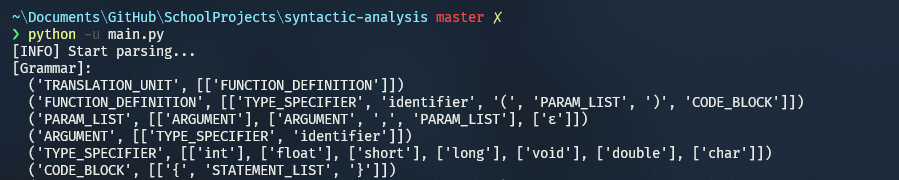
\includegraphics[width=\linewidth]{images/grammar.png}
  \caption{文法的输入字典(部分)}
  \label{fig:figure2}
\end{figure}

可以看到,我们将文法 Grammar 按照上面 3.2.2 中的描述进行了存储,以列表的形式进行访问。

\subsubsection{终结符和非终结符号}

\begin{figure}[h]
  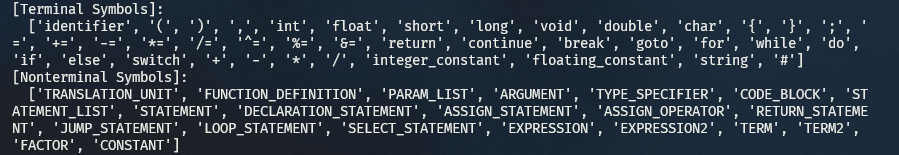
\includegraphics[width=\linewidth]{images/term_non.png}
  \caption{终结符和非终结符}
  \label{fig:figure3}
\end{figure}

我们将文法进行遍历,得到了如上的终结符和非终结符列表。

\subsubsection{First 和 Follow 集合(部分)}

\begin{figure}[h]
  \begin{subfigure}{\textwidth}
    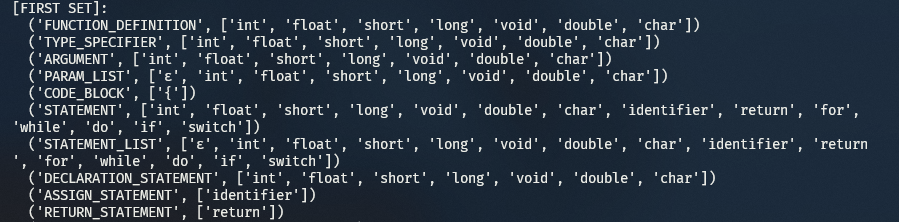
\includegraphics[width=\linewidth]{images/first.png}
    \caption{First 集合}
  \end{subfigure}
  \begin{subfigure}{\textwidth}
    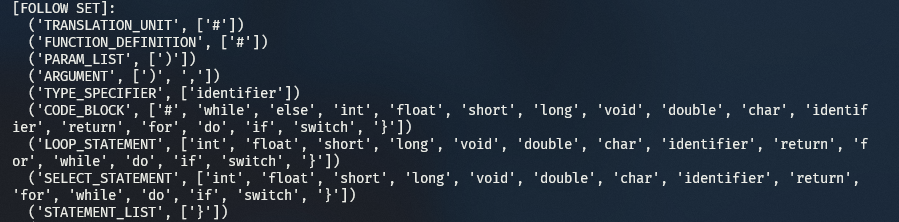
\includegraphics[width=\linewidth]{images/follow.png}
    \caption{Follow 集合}
  \end{subfigure}
  \caption{First 和 Follow 集合(部分)}
  \label{fig:figure4}
\end{figure}

我们接下来,就会得到构建 LL(1) 分析表所需的 First 和 Follow 集合。

\subsubsection{LL(1) 分析表的构建}
\begin{figure}[H]
  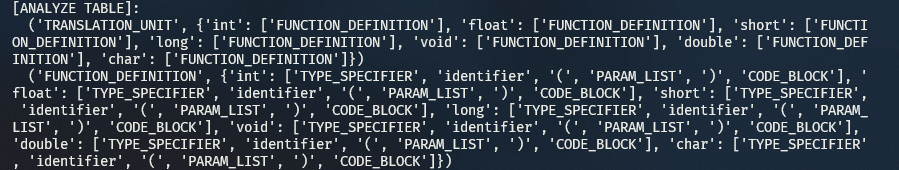
\includegraphics[width=\linewidth]{images/ll1_table.png}
  \caption{LL(1) 分析表(部分)}
  \label{fig:figure5}
\end{figure}

我们通过 First 和 Follow 集合就可以得到 LL(1) 分析表,如图 \ref{fig:figure5} 所示,我将 LL(1) 分析表通过字典的形式进行存储,以第一个单元格为例:

\begin{table}[H]
  \centering
  \caption{LL(1) 分析表第一个单元格}
  \label{tab:firstcell}
  \begin{tabular}{@{}c|c@{}}
  \toprule
   & int \\ \midrule
  TRANSLATION\_UNIT & TRANSLATION\_UNIT $\rightarrow$ FUNCTION\_DEFINITION \\ \bottomrule
  \end{tabular}
\end{table}

我将其表示为:

\begin{verbatim}
('TRANSLATION_UNIT', {'int': ['FUNCTION_DEFINITION'] ... })
\end{verbatim}

这样的表示形式更加方便后面对 LL(1) 分析表进行查表操作。

\subsection{语法树的生成}
\subsubsection{对输入串分析的输出}
\begin{figure}[h]
  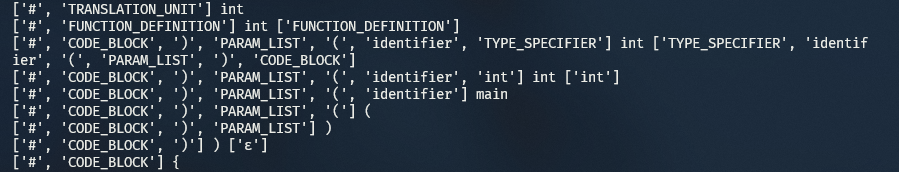
\includegraphics[width=\linewidth]{images/parse.png}
  \caption{LL(1) 分析器分析过程的大致输出(部分)}
  \label{fig:figure6}
\end{figure}

可以看到,我将分析过程的每次入栈、出栈都进行了按步骤的输出。每一行输出的格式为“分析栈栈内元素、当前输入串输入元素、所使用的产生式(后半部分)”。以第二行为例子:

\begin{table}[H]
  \centering
  \caption{分析过程第二行输出}
  \label{tab:parseoutput}
  \begin{tabular}{@{}c|c|c@{}}
  \toprule
  分析栈 & 输入字符 & 所使用的产生式 \\ \midrule
  {[}'\#', 'FUNC\_DEF'{]} & int & TRANS\_UNIT $\rightarrow$ FUNC\_DEF \\ \bottomrule
  \end{tabular}
\end{table}

\subsubsection{得到语法树并输出为 XML 文件}
\begin{figure}[h]
  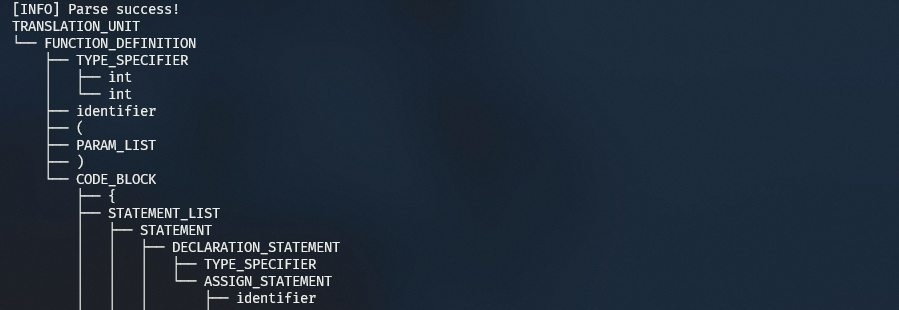
\includegraphics[width=\linewidth]{images/parsetree.png}
  \caption{分析得到的语法树(部分)}
  \label{fig:figure7}
\end{figure}

\begin{figure}[h]
  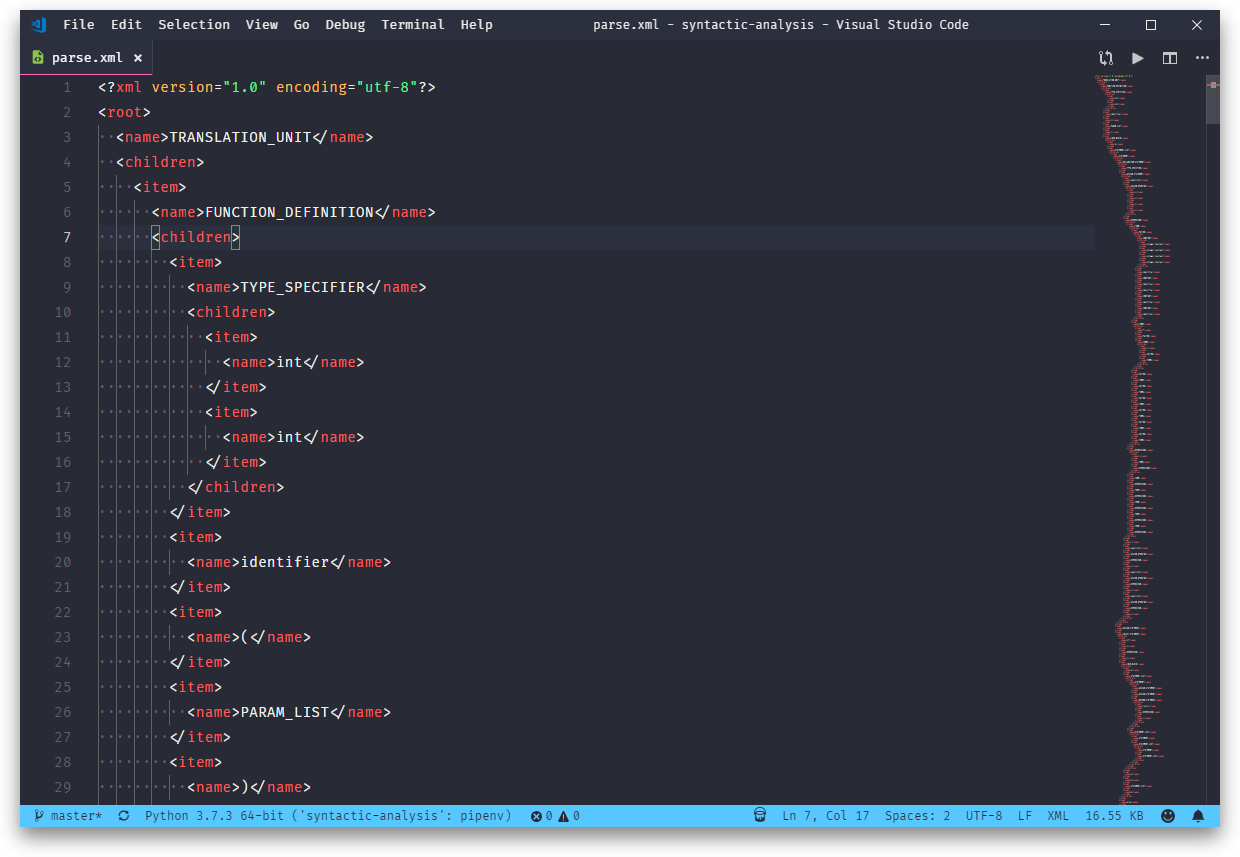
\includegraphics[width=\linewidth]{images/xml.png}
  \caption{通过语法树生成 XML 文件(部分)}
  \label{fig:figure8}
\end{figure}

\section{实验心得体会}
通过本次实验,我不仅更加熟悉了语法分析的具体过程,对自上而下的语法分析过程更加了解,还对 C 语言的文法描述、LL(1) 分析法的具体过程以及通过 LL(1) 分析表处理输入串的过程有了全新的认识。我在本次实验中,通过自己的扩展,处理得到了一个相对清晰的 C 语言 LL(1) 文法子集,利用 Python 构建了 C 语言的语法分析器,并成功的通过 LL(1) 分析器得到了一段 C 语言代码的语法分析树。

在本次实验中,我遇到最大的难题是对文法的处理。只有选取合适的数据结构,我才能更加方便的处理 C 语言的文法集合,也更加方便后续利用 LL(1) 分析表构建语法分析树的遍历过程。

与此同时,我通过本次实验的学习,还对 LL(1) 语法分析法、递归下降分析法以及 LR 语法分析法都有了全新的了解。总体来说,我收获颇丰。

\end{document}